\chapter{Analisi progettuale}
\label{ch:analisi progettuale}

In questo progetto si cerca di sviluppare un sistema per verificare in modo robusto la similarità tra password di un utente, in modo da evitare di utilizzare varianti di password precedenti, e garantire maggiore sicurezza di uno o più account.
A tal proposito sono stati condotti esperimenti che, per controllare la similarità tra password, utilizzavano word embedding di parole. In questo lavoro di tesi è stato preso come riferimento il paper di Bijeeta  et alii~\cite{bijeeta}.

\section{Modelli di similarità tra password basati sulle reti neurali}
\label{sec:modelli di similarita tra password basati sulle reti neurali}
Solitamente le metriche che misurano la robustezza di password non tengono conto della cronologia delle password passate di un utente.
Ciò può costituire un problema sia se si effettua un attacco contro un utente, sia per proteggerlo:
\begin{itemize}
    \item Durante un attacco, si considerano determinate password note grazie a leak, tuttavia non è presente un approccio flessibile che elabori varianti di password di un determinato utente.
    \item Non è presente un meccanismo che avverta l'utente del potenziale pericolo causato dal riutilizzo di password.
\end{itemize}
Per questo motivo, nel paper riferimento di Bijeeta et alii~\cite{bijeeta} sono stati utilizzate due tipologie di reti neurali:
\begin{itemize}
    \item Per l'attacco è stato sviluppato un modello di rete neurale ricorrente, noto come pass2path.
    \item Per la difesa sono stati utilizzate tecniche di Natural Language Processing, in particolare modelli di word embedding, i quali generano una corrispondenza tra parole e vettori, mantenendo proprietà semantiche della password originale, come la similarità.
\end{itemize}

\section{Prerequisiti}
\label{sec:prerequisiti}
Per la creazione dei due modelli visti precedentemente, è stato utilizzato un leak disponibile sul Deep Web, di dimensione pari a 45 GB e contenente 1.4 miliardi di coppie mail-password appartenenti ad account su social come LinkedIn, MySpace, Badoo, Yahoo, Zoosk; successivamente è stato filtrato nel seguente modo:

\begin{itemize}
    \item sono state rimosse le stringhe che contenevano 20 o più caratteri esadecimali;
    \item sono stati rimossi hash non decodificati;
    \item sono state rimosse le password più lunghe di 50 caratteri o più corte di 3 che contenevano caratteri non ASCII;
    \item sono stati rimossi 4528 utenti associati a centinaia di password, poiché è molto improbabile che siano account veri.
\end{itemize}

Dal risultato del processo di filtraggio sono stati osservati i seguenti punti:
\begin{itemize}
    \item la password 123456 è stata utilizzata dal 0.9\% degli utenti;
    \item più dell'88\% di password hanno una lunghezza compresa tra 6 e 12 caratteri;
    \item l'80\% delle password contiene solo caratteri minuscoli.
\end{itemize}

\begin{figure}[h]
    \centering
    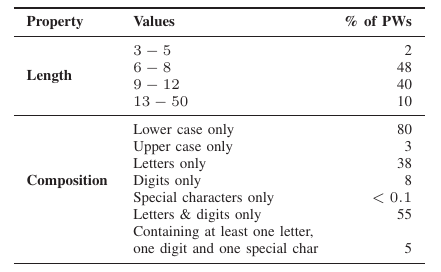
\includegraphics[width=11cm]{./immagini/pulizia_dataset_bijeeta.png}
    \label{pulizia dataset}
    \caption{La distribuzione della lunghezza delle password e della loro composizione dopo la pulizia del dataset~\cite{bijeeta}}
\end{figure}



\section{Strategie di attacco: pass2path}
\label{sec:pass2path}
\subsection{Euristiche e appartentenza di password}
\label{sec:euristiche e appartenenza di password}
Una volta ottenuto il dataset, è necessario capire a quali persone appartengono gli account. A tal proposito vengono proposte tre euristiche:
\begin{itemize}
    \item \textbf{Basata su email:} gli utenti vengono identificati solo dalla email. Ciascuna email appartiene a un solo utente.
    \item \textbf{Basata sugli username:} si considera la stringa che precede \texttt{@} nell'indirizzo email. Un utente può possedere più mail, tutte identificate dalla stringa che precede \texttt{@}.
    \item \textbf{Basata su un metodo misto:} considera sia gli username che le email. Due email sono considerate connesse tra loro se hanno almeno una password in comune e se le mail connesse tra loro sono associate allo stesso username.
\end{itemize}
Per potere effettuare migliori test sul dataset sono stati rimossi gli utenti che avevano meno di due password associate allo stesso account.

Il dataset successivamente viene diviso in due parti: training set e test set (in rapporto 80\%-20\% ). Nel paper la fase di training utilizza soltanto il dataset relativo all'euristica basata sulle email, mentre per la fase di testing si utilizza sia l'euristica basata sulle email sia quella mista.

\subsection{Introduzione a pass2path}
\label{sec:intro pass2path}
Pass2path è un modello di rete neurale che consente di creare password in grado di compromettere più del 48\% degli utenti in meno di mille tentativi. Il successo di questo modello è dovuto al riutilizzo della stessa password o di varianti di password da parte dell'utente.
Per svilupparlo si è tenuto conto della sequenza di trasformazioni $\tau_1...\tau_n $, nota come \emph{percorso} che consente, a partire dalla password  $\tilde{w}$, di produrre la nuova password $w$.


Le modifiche sono rappresentate da una unità di misura $\tau\in \mathcal{T}$, che specifica in che posizione e quale tipo di variazione applicare a una password.
\\
$\tau$ è composto da una tripletta  $\{e, c', l\}$:
\begin{itemize}
    \item $e$ rappresenta una modifica da apportare;
    \item $c'$ rappresenta un carattere o una stringa vuota;
    \item $l$ rappresenta la posizione della modifica della password.
\end{itemize}

Le modifiche vengono classificate in tre tipologie:
\begin{itemize}
    \item \texttt{sub} (sostituzione);
    \item \texttt{ins} (inserimento);
    \item \texttt{del} (cancellazione).
\end{itemize}

Se si considera $c'$ sono presenti due situazioni:
\begin{itemize}
    \item \texttt{ins} e \texttt{sub}: $c'$ rappresenta il carattere o la stringa vuota;
    \item \texttt{del}: è sempre una stringa vuota.
\end{itemize}

Per ricavare il percorso tra due password, si considera quello più corto, nel seguente ordine decrescente di preferenza:
\begin{enumerate}
    \item \texttt{del};
    \item \texttt{ins};
    \item \texttt{sub}.
\end{enumerate}

Le varie trasformazioni del percorso vengono ordinate in base alla posizione della modifica.

Ad esempio, il percorso da \texttt{cats} a \texttt{kates} (distanza di modifica pari a 2) è:
\begin{center}
    $path = \{(sub , k^\prime , 0), (ins , e^\prime , 3)\}$
\end{center}

\subsection{Come allenare pass2path}
\label{sec:allenamento pass2path}
Prima di allenare pass2path è necessario tradurre ciascuna password come sequenza di tasti premuti su una \emph{tastiera americana ANSI}. La codifica dei tasti premuti è la seguente:
\begin{itemize}
    \item Per rappresentare una sola lettera maiuscola all'interno di una parola si pone \texttt{<s>} (che rappresenta la pressione del tasto \texttt{SHIFT}) prima della lettera, che viene lasciata minuscola. Ad esempio \texttt{Ciao} viene tradotto come \texttt{<s>ciao}.
    \item se si hanno più lettere maiuscole consecutive seguite da lettere minuscole si pone \texttt{<c>} (che rappresenta la pressione del tasto \texttt{CAPS LOCK}) prima e dopo la sequenza di lettere maiuscole, che viene lasciata minuscola. Per esempio \texttt{PASSword} viene tradotto come \texttt{<c>pass<c>word}.
    \item Nel caso di una sequenza di lettere maiuscole che si conclude alla fine della parola basta porre \texttt{<c>} all'inizio della sequenza. Per esempio \texttt{PASSWORD} viene tradotto come \texttt{<c>password} e \texttt{passWORD} come \texttt{pass<c>word}.
    \item Se si hanno caratteri speciali ASCII 128 si pone \texttt{<s>} davanti al carattere.
    \\
    Quest'ultimo viene tradotto come il tasto che viene premuto insieme a \texttt{SHIFT}.
    Per esempio \texttt{PASSWORD!} viene rappresentata come \texttt{<c>password<s>1}, dato che \texttt{1} viene premuto insieme a \texttt{SHIFT} e \texttt{Hello@!!} viene tradotto come
    \\
    \texttt{<s>hello<s>2<s>1<s>1}.
\end{itemize}

\begin{figure}[h]
    \centering
    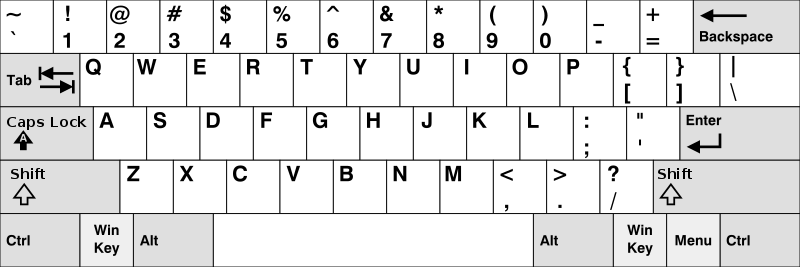
\includegraphics[width=15cm]{./immagini/US_keyboard_layout.png}
    \label{US layout}
    \caption{\href{https://upload.wikimedia.org/wikipedia/commons/thumb/5/51/KB_United_States-NoAltGr.svg/800px-KB_United_States-NoAltGr.svg.png}{Layout della tastiera americana ANSI, fonte: Wikipedia}}
\end{figure}

Successivamente occorre trovare il percorso di transizioni  $\tau_1...\tau_n$ che consentano di trasformare la password $\tilde{w}$ in $w$.

Si è deciso di filtrare le password in base alla lunghezza del percorso, che deve tenere conto anche della modifica di una password basata sulla sequenza di tasti premuti. Sono state eliminate le password con un percorso di lunghezza superiore a $\delta$.

Per allenare pass2path si utilizza il dataset di training basato sulle email.
Si utilizzano due reti neurali ricorrenti (RNN) per costruire un auto-encoder~\cite{Sherstinsky_2020}.

\subsection{Efficacia d'attacco con configurazioni non ripetute}
\label{sec:attacco conf non ripetute}
Per verificare l'efficacia di attacco della rete si utilizza il dataset di test delle email, con password da indovinare $w$ diverse dalla originale $\tilde{w}$.
Con configurazioni non ripetute, pass2path riesce in meno di 100 stime a ricavare
il 13\% delle password, impiegando 4 ore in tutto (Intel i9 e 128 GB di RAM, su un singolo thread).
\begin{figure}[h]
    \centering
    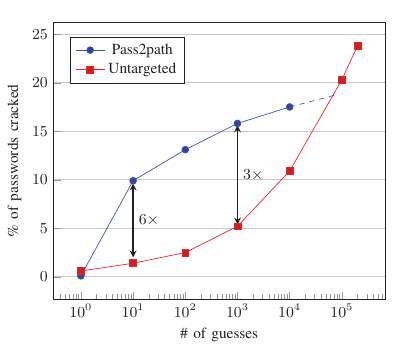
\includegraphics[width=10cm]{./immagini/pass2path.png}
    \label{pass2path}
    \caption{Pass2path riesce a indovinare in meno di mille tentativi una percentuale più alta di password, rispetto ad attacchi non mirati. Questi ultimi risultano efficaci soltanto se sono richiesti più di 1000 tentativi~\cite{bijeeta}}
\end{figure}

\subsection{Efficacia d'attacco con configurazioni ripetute}
\label{sec:attacco conf ripetute}
Per verificare l'efficacia di un attacco della rete, in caso di password da indovinare $w$ simile alla originale $\tilde{w}$, si utilizza il test set del dataset misto, in cui si è osservato che il 40\% delle password vengono riutilizzate dagli utenti, rendendoli facili bersagli.

Come primo attacco viene utilizzata la password $\tilde{w}$, in modo da verificare il suo riutilizzo senza varianti, mentre i restanti $q - 1$ vengono svolti in accordo alla tecnica di attacco scelta. Confrontando con altri modelli utilizzati, il migliore risultato è stato ottenuto da pass2path, compromettendo metà degli utenti (48.3\%) in al massimo mille tentativi.
Si è osservato che con password riutilizzate, aumentano le probabilità di indovinare la password con pass2path.
Inoltre è importante sottolineare che gli attacchi di tipo non mirato (untargeted) ottengono migliori performance se vengono eseguiti più di 1000 tentativi; al contrario pass2path è il migliore approccio nel caso in cui si proceda con un numero minore.


I ricercatori hanno anche eseguito un vero e proprio attacco all'interno della loro università (Cornell University), in modo da potere testare su password diverse da quelle del dataset, ovvero appartenenti a studenti e professori. Il migliore risultato è stato ottenuto da pass2path, che in meno di 1000 tentativi è riuscito a scoprire la password del 8,4\% degli account~\cite{bijeeta}.


\section{Difesa}
\label{sec:difesa}
\subsection{Difesa da attacchi a dizionario mirati}
\label{sec:difesa attacchi mirati}
Diversi studi mostrano che cambiare password non protegge completamente un utente dagli attacchi~\cite{google}~\cite{hypr}.
Nel paper viene illustrato il concetto di PPSM (Personalized password strength meters), che sfruttano modelli preallenati di word embedding per dimostrare la sicurezza di una password.
In questo modo si possono prevenire attacchi che sfruttano varianti di password presenti in data breach.

\subsection{Personalized password strength meters}
\label{sec:ppsm}
Un PPSM può essere utilizzato con lo scopo di dare un giudizio in tempo reale all'utente sulla sicurezza delle password durante la selezione.
Il funzionamento è il seguente:
\begin{itemize}
    \item vengono considerati in input una potenziale password e un set di password associate all'utente trovate in un data leak;
    \item vengono utilizzati due possibili criteri come output:
    \begin{itemize}
        \item \textbf{guess rank}, ovvero il numero di tentativi di una tipologia di attacco fatti prima di indovinare la password;
        \item \textbf{percentuale di similarità}, ovvero la somiglianza tra la potenziale password e la password associata all'utente.
    \end{itemize}
\end{itemize}

Un possibile modo di ottenere il guess rank è basarsi su pass2path, in modo da evitare che un utente usi una password simile a quella trovata in un data breach; tuttavia prevedere password risulta costoso (dato che si considera un modello di generazione di password come pass2path) e, nel caso in cui si vogliano inviare i risultati via rete, viene occupata molta banda.

Si è osservato che risulta più efficiente e meno costoso assegnare punteggi che rappresentano la sicurezza di una password rispetto ai guess rank~\cite{bijeeta}.

\subsection{Realizzazione di un PPSM}
\label{sec:realizzazione ppsm}
Sotto al PPSM si trova un classificatore binario $C$ che prende in input una password candidata $w$ e una password nota da un leak $\tilde{w}$ e restituisce 0 se $w$ è indovinabile in meno di 1000 tentativi a partire da $\tilde{w}$, 1 altrimenti.
Per costruire tale classificatore è necessario utilizzare tecniche di word-embedding.

\subsection{Similarità tra password via word embedding}
\label{sec:similarita via word embedding}
Si definisce word embedding la tecnica di mappatura di un insieme di parole in uno spazio vettoriale d-dimensionale (solitamente con d che vale 100 o 200 o 300).

In questo modo vengono preservate le proprietà semantiche delle parole, come ad esempio la loro similarità: ad esempio, se due parole compaiono spesso nello stesso contesto, le loro rappresentazioni vettoriali avranno una distanza ridotta.

In particolare, nel problema in esame, la tecnica di word embedding viene applicata alle password: due password risultano simili se vengono scelte spesso dallo stesso utente. Ciò permette di stabilire quanto una password sia sicura, considerando tutte le password precedentemente scelte dall'utente, e di fornire un punteggio (ovvero la percentuale di similarità).

A tal scopo, per costruire un password embedding model, viene utilizzato FastText, che impara la similarità dividendo la parola in una collezione di contesti, definiti come piccole sequenze di parole note come \emph{n-gram}. Le parole che appaiono spesso insieme nello stesso contesto vengono definite simili.

\subsection{Allenamento di Fasttext}
\label{sec:allenamento fasttext}
Per l'allenamento del modello di FastText vengono considerati i seguenti parametri:

\begin{itemize}
    \item \textbf{Dimensione del vettore}: impostata a 100, poiché l'allenamento del modello così risulta più rapido rispetto al parametro di default a 300.
    \item \textbf{Subsampling}: ignora le password che ricorrono più frequentemente. Impostato a $10^{-3}$, poiché non si vogliono password con più di 1000 occorrenze.
    \item \textbf{Dimensione minima degli ngram}: impostata a 1, in modo che possano essere costruiti embedding per password mai viste durante l'allenamento.
    \item \textbf{Dimensione massima degli ngram}: impostata a 4, dato che le parole presenti nel dataset hanno come minimo 4 caratteri.
\end{itemize}
\subsection{Classificazione delle password}
\label{sec:classificazione password}
Per classificare le password viene utilizzato un classificatore binario che restituisce 0 se le password sono simili tra loro, superando una soglia $\alpha$ di similarità decisa prima della misurazione, 1 altrimenti.

Una password risulta vulnerabile se, data una password $w$, essa viene indovinata in meno di 1000 tentativi a partire dalla password $\tilde{w}$, utilizzando come euristica pass2Path.
Per determinare la soglia $\alpha$, vengono considerati $10^5$ utenti dal dataset di test delle email e per ciascun utente vengono sorteggiate due password dalla collezione di password associati a essi. Una delle due password (la scelta della password è arbitraria) viene considerata come la nuova password da indovinare $w$, mentre l'altra password $\tilde{w}$ rappresenta la password trovata in un leak.
\begin{figure}[h!]
    \centering
    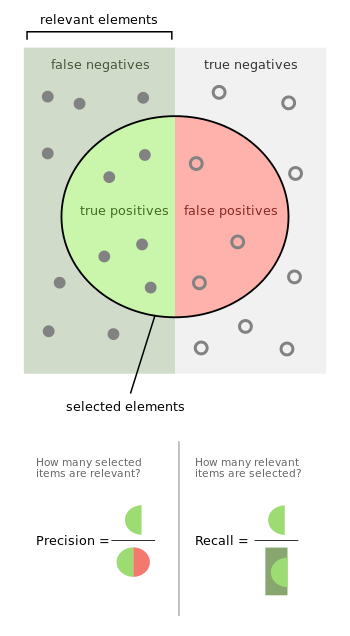
\includegraphics[width=7cm]{./immagini/precisionrecall.png}
    \caption{\href{https://upload.wikimedia.org/wikipedia/commons/2/26/Precisionrecall.svg}{Definizione grafica di precision e recall, fonte: Wikipedia}}
    \label{precision recall}
\end{figure}
\FloatBarrier
Vengono definiti due parametri per la scelta di $\alpha$:
\begin{itemize}
    \item \textbf{Precision}: rappresenta quanti veri positivi sono stati rilevati su un totale composto da veri positivi e falsi positivi.
    \item \textbf{Recall}: rappresenta il numero effettivo di elementi positivi che sono stati rilevati su un totale di falsi negativi e veri positivi.
\end{itemize}
In particolare, nel caso in esame:
\begin{itemize}
    \item per vero positivo si intende una coppia di password simili correttamente rilevate come tali;
    \item per falso positivo si intende una coppia di password diverse erroneamente rilevate come simili;
    \item per falso negativo si intende una coppia di password simili erroneamente non rilevate come tali.
\end{itemize}
Un valore di precision basso implica una imprecisa distinzione tra password simili e password non simili; un valore di recall basso invece comporta avere molte password simili non rilevate come tali.

Nel paper di riferimento di Bijeeta et alii~\cite{bijeeta} viene considerato un valore di recall molto alto (99\%) e una percentuale di precision nettamente più bassa (60\%). Per questo motivo $\alpha$ è stato posto a $0.5$.

\begin{figure}[h]
    \centering
    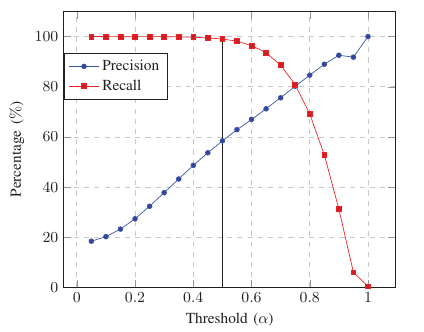
\includegraphics[width=11cm]{./immagini/precision_recall_paper_bijeeta.png}
    \label{precisionbijeeta}
    \caption{Precision e recall di Bijeeta et al.~\cite{bijeeta}}
\end{figure}
\subsection{Modelli compressi di word embedding}
\label{sec:modelli compressi word embedding}
Il modello prodotto da Bijeeta et alii~\cite{bijeeta} è stato successivamente compresso, in modo da ridurre la dimensione da 1.5 GB a 3 MB, senza che la qualità delle performance venisse ridotta, mediante tecniche di quantizzazione.
Per la produzione del modello compresso si è tenuto conto del parametro $\eta$ che determina il rapporto di compressione. Per la valutazione della compressione, sono stati prodotti più modelli in base a differenti valori $\eta$; infine è stato scelto il modello con $\eta=5$ e dimensione complessiva di 3 MB, poiché il valore di recall non ha subito notevoli variazioni.
\begin{figure}[h]
    \centering
    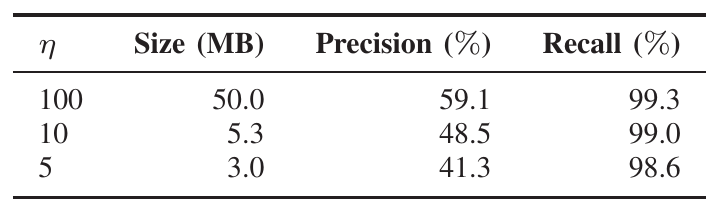
\includegraphics[width=9cm]{./immagini/compressed_model.png}
    \label{compressed_model}
    \caption{Precision e recall in base al rapporto di compressione $\eta$ del modello di Bijeeta et alii~\cite{bijeeta}}
\end{figure}
\section{Modifiche e analisi del progetto}
\label{sec:modifiche analisi del progetto}
Per questo progetto sono state effettuate diverse scelte:

\begin{itemize}
    \item Si è scelto di non implementare pass2path, per motivi di complessità e di costo in termini di testing;
    \item sono stati modificati i criteri di filtraggio del dataset per allenare il modello di word embedding;
    \item sono state utilizzate euristiche diverse rispetto a pass2path;
    \item sono stati modificati i parametri per allenare la rete neurale che ricava la similarità tra password.
\end{itemize}
